
%(BEGIN_QUESTION)
% Copyright 2012, Tony R. Kuphaldt, released under the Creative Commons Attribution License (v 1.0)
% This means you may do almost anything with this work of mine, so long as you give me proper credit

En {\it boiling-water reactor} (BWR) i et kjernekraftverk bruker varmen fra reaktorkjernen til å koke vann til damp, som driver dampturbin og generator:

$$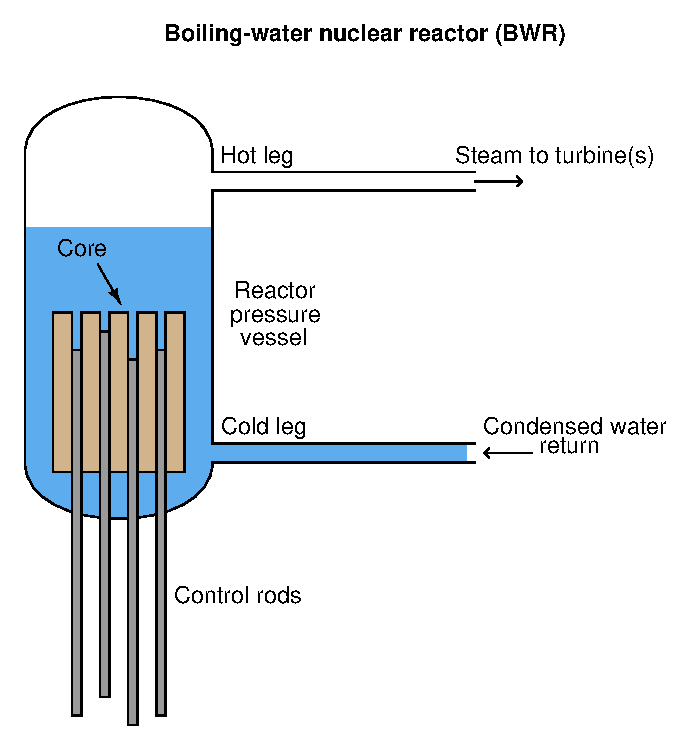
\includegraphics[width=15.5cm]{i01018x01.eps}$$

Det er kritisk at kjernen holdes helt neddykket i vann.

\vskip 10pt

Anta målt temperatur og trykk på en BWR er 780 $^{o}$F og 495 PSIG. Bruk damptabell og avgjør om kjernen er dekket (neddykket) eller avdekket (eksponert).

\underbar{file i01018}
%(END_QUESTION)





%(BEGIN_ANSWER)

Mettet damptemperatur ved 505 PSIG (høyere enn 495 PSIG) er 471 $^{o}$F. Siden 780 $^{o}$F er mye høyere, er dampen i hot leg superopphetet. Det betyr at kjernen tilfører varme etter at vannfasen er borte lokalt: kjernen er avdekket.
 
\vskip 10pt

Dette er en svært alvorlig situasjon.

%(END_ANSWER)





%(BEGIN_NOTES)

Under Three Mile Island-ulykken ble lignende observasjoner tolket som avdekket kjerne.

%INDEX% Physics, heat and temperature: saturated steam pressure versus temperature
%INDEX% Physics, heat and temperature: steam table
%INDEX% Physics, heat and temperature: superheated steam

%(END_NOTES)

